%%%%%%%%%%%%%%%%%%%%%%%%%%%%%%%%%%%%%%%%%
% Masters/Doctoral Thesis
% LaTeX Template
% Version 2.5 (27/8/17)
%
% This template was downloaded from:
% http://www.LaTeXTemplates.com
%
% Version 2.x major modifications by:
% Vel (vel@latextemplates.com)
%
% This template is based on a template by:
% Steve Gunn (http://users.ecs.soton.ac.uk/srg/softwaretools/document/templates/)
% Sunil Patel (http://www.sunilpatel.co.uk/thesis-template/)
%
% Template license:
% CC BY-NC-SA 3.0 (http://creativecommons.org/licenses/by-nc-sa/3.0/)
%
%%%%%%%%%%%%%%%%%%%%%%%%%%%%%%%%%%%%%%%%%

%----------------------------------------------------------------------------------------
%	PACKAGES AND OTHER DOCUMENT CONFIGURATIONS
%----------------------------------------------------------------------------------------

% Pages (from the internal page numbering) to be printed in color - 3, 4, 5, 11, 12, 13, 14, 17, 18, 20, 21, 23, 25, 27.

\documentclass[
hidelinks,
12pt, % The default document font size, options: 10pt, 11pt, 12pt
oneside, % Two side (alternating margins) for binding by default, uncomment to switch to one side
english, % ngerman for German
doublespacing, % Single line spacing, alternatives: onehalfspacing or singlespacing
%draft, % Uncomment to enable draft mode (no pictures, no links, overfull hboxes indicated)
%nolistspacing, % If the document is onehalfspacing or doublespacing, uncomment this to set spacing in lists to single
%liststotoc, % Uncomment to add the list of figures/tables/etc to the table of contents
%toctotoc, % Uncomment to add the main table of contents to the table of contents
%parskip, % Uncomment to add space between paragraphs
%nohyperref, % Uncomment to not load the hyperref package
headsepline, % Uncomment to get a line under the header
%chapterinoneline, % Uncomment to place the chapter title next to the number on one line
%consistentlayout, % Uncomment to change the layout of the declaration, abstract and acknowledgements pages to match the default layout
]{MastersDoctoralThesis} % The class file specifying the document structure

\usepackage[utf8]{inputenc} % Required for inputting international characters
\usepackage[T1]{fontenc} % Output font encoding for international characters
\usepackage{subcaption}
\usepackage{mathpazo} % Use the Palatino font by default
\usepackage{booktabs}
\usepackage{colortbl}
\usepackage[final]{pdfpages}
\usepackage{xcolor}
\usepackage{balance}
\usepackage{epigraph}
\usepackage{alltt} % for code snippet
\usepackage{listings}
\usepackage{hyperref}
\usepackage{amsmath}
\usepackage{macros}
\usepackage{mathtools}
\usepackage{float}
\usepackage{newtxmath}
\usepackage{polski}
\usepackage[backend=bibtex,style=authoryear,natbib=true]{biblatex} % Use the bibtex backend with the authoryear citation style (which resembles APA)
%\usepackage[backend=bibtex,style=authoryear,natbib=true,backref=true]{biblatex} % use this line instead of the previous one if you want to use back references

\addbibresource{biblio.bib} % The filename of the bibliography


\usepackage[autostyle=true]{csquotes} % Required to generate language-dependent quotes in the bibliography

%----------------------------------------------------------------------------------------
%	MARGIN SETTINGS
%----------------------------------------------------------------------------------------

\geometry{
	paper=a4paper, % Change to letterpaper for US letter
	inner=4.0cm, % Inner margin
	outer=3.0cm, % Outer margin
	bindingoffset=.5cm, % Binding offset
	top=2.5cm, % Top margin
	bottom=2.5cm, % Bottom margin
	%showframe, % Uncomment to show how the type block is set on the page
}

%----------------------------------------------------------------------------------------
%	THESIS INFORMATION
%----------------------------------------------------------------------------------------

\thesistitle{Manifold Structure of High-Dimensional Data in Visual Perception} % Your thesis title, this is used in the title and abstract, print it elsewhere with \ttitle
\supervisor{Dr/Pr. FirstName \textsc{LastName}} % Your supervisor's name, this is used in the title page, print it elsewhere with \supname
\examiner{Dr/Pr. FirstName \textsc{LastName}} % Your examiner's name, this is not currently used anywhere in the template, print it elsewhere with \examname
\degree{B.Sc (Hons)} % Your degree name, this is used in the title page and abstract, print it elsewhere with \degreename
\author{\textsc{Zhang} Liu} % Your name, this is used in the title page and abstract, print it elsewhere with \authorname
\addresses{} % Your address, this is not currently used anywhere in the template, print it elsewhere with \addressname

\subject{Mathematical, Computational and Statistical Sciences} % Your subject area, this is not currently used anywhere in the template, print it elsewhere with \subjectname
\keywords{manifold learning, recurrent neural networks, computational vision, harmonic analysis} % Keywords for your thesis, this is not currently used anywhere in the template, print it elsewhere with \keywordnames
\university{\href{https://www.yale-nus.edu.sg/}{Yale-NUS College}} % Your university's name and URL, this is used in the title page and abstract, print it elsewhere with \univname
\department{{}} % Your department's name and URL, this is used in the title page and abstract, print it elsewhere with \deptname
\group{{}} % Your research group's name and URL, this is used in the title page, print it elsewhere with \groupname
\faculty{{}} % Your faculty's name and URL, this is used in the title page and abstract, print it elsewhere with \facname

\AtBeginDocument{
\hypersetup{colorlinks=false}
\hypersetup{pdftitle=\ttitle} % Set the PDF's title to your title
\hypersetup{pdfauthor=\authorname} % Set the PDF's author to your name
\hypersetup{pdfkeywords=\keywordnames} % Set the PDF's keywords to your keywords
\hypersetup{hypertexnames=true}
}

\begin{document}

\frontmatter % Use roman page numbering style (i, ii, iii, iv...) for the pre-content pages

\pagestyle{plain} % Default to the plain heading style until the thesis style is called for the body content

%----------------------------------------------------------------------------------------
%	TITLE PAGE
%----------------------------------------------------------------------------------------

\begin{titlepage}
% Fill out the titlepage.docx document, then save it as a pdf for inclusion here
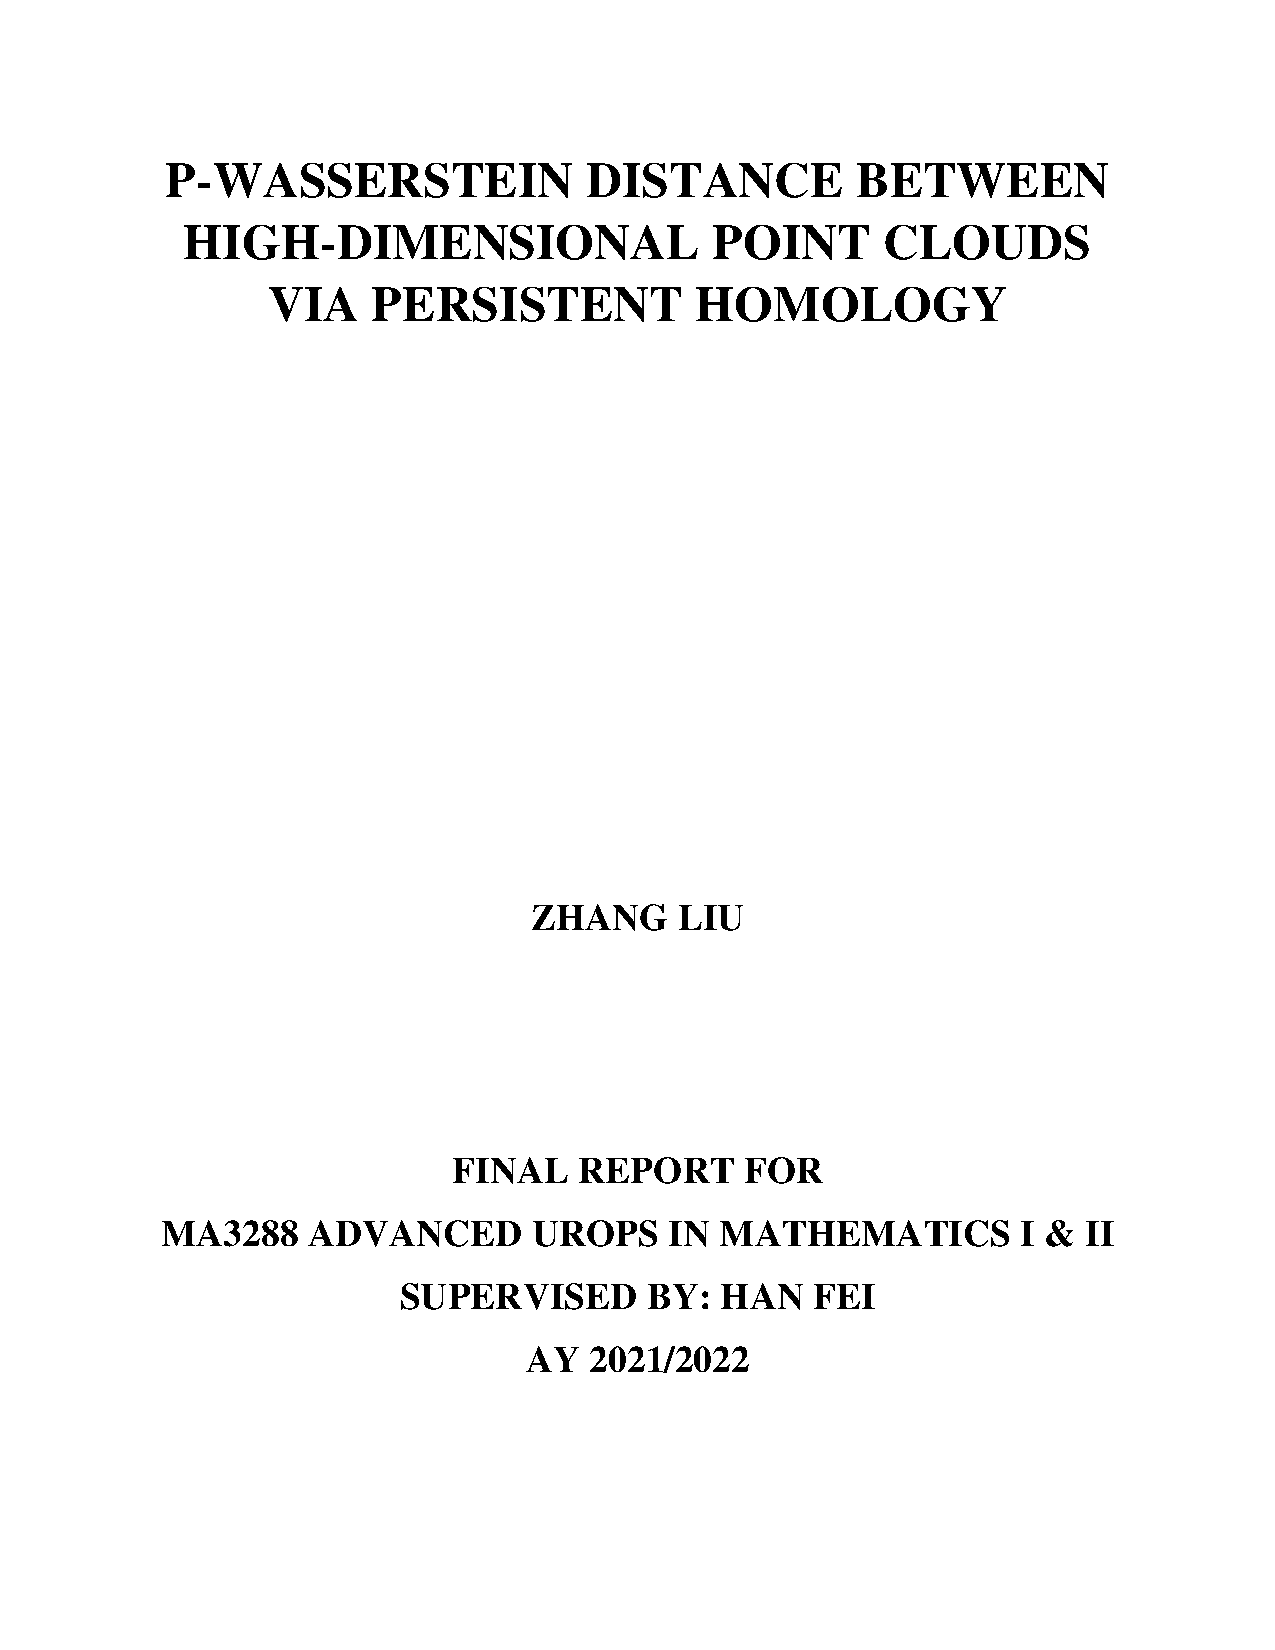
\includepdf[pages=-,pagecommand={},width=\textwidth]{titlepage.pdf}

\end{titlepage}

%----------------------------------------------------------------------------------------
%	DECLARATION & CONSENT
%----------------------------------------------------------------------------------------

% print, sign, and scan the declaration form, then include it here
\includepdf[pages=-,pagecommand={},width=\textwidth]{declaration.pdf}

%----------------------------------------------------------------------------------------
%	ACKNOWLEDGEMENTS
%----------------------------------------------------------------------------------------

\begin{acknowledgements}
\addchaptertocentry{\acknowledgementname} % Add the acknowledgements to the table of contents
    I would like to thank my mentors Prof.~Steven W. Zucker and Dr.~Luciano Dyballa for their generous guidance and advice. They have made possible the many serendipitous moments in this project. I am also grateful for Yale-NUS CIPE for their general support and for my advisor Prof.~Francesca Spagnuolo for her encouragement throughout my mathematical career.
\end{acknowledgements}

%----------------------------------------------------------------------------------------
%	ABSTRACT PAGE
%----------------------------------------------------------------------------------------

\begin{abstract}
\addchaptertocentry{\abstractname} % Add the abstract to the table of contents
\textbf{Key words: \keywordnames}

This work builds on a long line of research aiming to develop more accurate mathematical and computational models of the visual system. It has recently been shown that feed-forward neural networks turn out to be inaccurate models for the brain. We focused on a related question that has not been investigated: how is the structure of recurrent and transformer neural networks related to that of neurobiological networks (in the mouse visual cortex)?

We first build the biological and artificial neuron tensors using experimental neural spiking data and numerical simulations on recurrent and transformer neural networks. Using tensor component analysis, we discover which groups of neurons respond similarly to which stimuli input. Since these groups are likely not independent, we use the non-linear dimensionality reduction method, diffusion maps, to infer a manifold of neurons. This manifold structure implies a functional network (represented by the discrete data graph underlying the continuous manifold) and thus reflects both the neural circuit connections and the neuron’s role in those circuits. Comparing the manifold structures of biological and artificial neural networks allows us to make precise inferences about similarities and differences in their respective functional circuits. 

\end{abstract}


%----------------------------------------------------------------------------------------
% CONTRIBUTIONS
%----------------------------------------------------------------------------------------

% \chapter{Claims}
%
% This paper presents the following original contributions:
%
% \begin{enumerate}
% 	\item A hardware device for haptic sensory substitution along with designs for the construction of such a system.
% 	\item Two implementations of sensory substitution using haptic feedback, continuous and delayed feedback-based spatial navigation tasks, each of which include:
% 		\begin{enumerate}
% 			\item a front-end for providing visual input to the user during the training phase with useful readouts to the researcher,
% 			\item a transmission protocol, which maps information from the task at hand (spatial coordinates, velocity information, etc) to time-based sensor actuation signals (20$^{\circ}$ on servo 1, 35$^{\circ}$ on servo 2, etc) in real-time.
% 		\end{enumerate}
% 	\item An evaluation framework for measuring the performance of a sensory substitution system, which provides sample tasks that can be used to standardise and compare performance across the board for future research.
% 	\item A review of existing hardware and software stacks as well as possible avenues for development based on the developed metrics.
% \end{enumerate}
%
% In addition, code for displaying results in real-time, modules for managing servo overload, network latency and other factors were also written by the author.

%----------------------------------------------------------------------------------------
%	QUOTATION PAGE
%----------------------------------------------------------------------------------------

% \vspace*{0.2\textheight}
%
% \noindent\enquote{\itshape Thanks to my solid academic training, today I can write hundreds of words on virtually any topic without possessing a shred of information, which is how I got a good job in journalism.}\bigbreak
%
% \hfill Dave Barry

\tableofcontents

%----------------------------------------------------------------------------------------
%	THESIS CONTENT - CHAPTERS
%----------------------------------------------------------------------------------------

\mainmatter 
\pagestyle{thesis}

\chapter{Chapter 0: Introduction} 
\label{Chapter0} 

\section{Historical Context}

\subsection{Hierarchy Models}

\par Hubel and Wiesel (1962) classified primary visual cortex (V1) neurons into simple cells and complex cells. The essential difference between the simple cells and complex cells is that the responses of simple cells are modulated by the spatial phase of a sine grating, whereas the responses of complex cells are largely phase invariant. In other words, as we progress from simple cells to complex cells, the neurons become selective for increasingly complex stimuli and at the same time become more tolerant to the exact position within their receptive fields. 

\par Based on this, a natural way to construct complex cells is to group responses from simple cells with the same orientation preference, but with different phase preferences.

\par This idea directly inspired the Neocognitron model:  S-cells are tuned to simple stimuli after a few operations (convolution) and then they are combined (by pooling through maximum or average) to form C-cells tuned to more complex stimuli. 

\par The Neocognitron model is among a myriad of hierarchical models of the visual system. They differ in their specific wiring, parameterizations, and the mathematical operations. But all of these models has a common basic structure, Hmax:

\begin{figure}[H]
\centering
    \includegraphics[width=7cm]{figures/models/hmax.png}
     \caption{An Intuitive Illustration of Hmax (Serre, 2014)}
\end{figure}

\par The figure below shows a systematic illustration of the general idea behind the hierarchical models:
\begin{figure}[H]
\centering
    \includegraphics[width=10cm]{figures/models/hierarchical-models.png}
     \caption{Illustration of the hierarchical models (Martinez and Alonso, 2003)}
\end{figure}

\par The possible advantages of hierarchical models are as follows:
\begin{itemize}
    \item If a visual recognition task can be decomposed into low-complexity learning tasks for each layer of a hierarchical learning machine, then each layer may require only a small number of training examples (Poggio and Smale, 2003).
    \item The lowest levels of the hierarchy may represent a dictionary of features that can be shared across multiple classification tasks (Geman, 1999), thus increasing efficiency.
\end{itemize}

\par There are also some known limitations of hierarchical models:
\begin{itemize}
    \item Hierarchical models assume that the computations at each successive stage being largely feedforward (Riesenhuber and Poggio, 1999; DiCarlo et al., 2012). This is limited because back-projections are also likely to be a key part of the visual system. 
    \item There remains a very broad distribution of tuning and receptive field sizes in all areas of the visual hierarchy. Hence, the anatomical hierarchy should be taken as an idealization and cannot be taken as a strict flowchart of visual information (Hegde and Felleman, 2007). 
    \par One particularly interesting piece of evidence: A close comparison of shape representation between V1, V2 and V4 also demonstrated a complex pattern of shape selectivity with significant deviation from strict hierarchical organization with some cells in V1 exhibiting more complex tuning than some cells in V4 (Hegde and Van Essen, 2007).
\end{itemize}


\subsection{Alternative Models}
\par Since Hubel and Wiesel (1962) proposed the classification of simple cells and complex cells, many other hierarchical models have been proposed for a more realistic representation for the cortical circuitry. Furthermore, new experimental and computational evidence provided serious alternatives to this hierarchical model, including parallel models and recurrent models (Martinez and Alonso, 2003). There are still many controversies and debates over which models best capture mechanisms of the visual system.

\subsubsection{Parallel Models}
\par The first strong evidence against the hierarchical model was the discovery that some complex cells, like simple cells, receive monosynaptic input from the thalamus (Hoffmann and Stone 1971). Based on this discovery, Hoffman and Stone proposed that both cell types, simple and complex, were generated in parallel by separate thalamocortical pathways (Hoffman and Stone 1971), as shown in diagram A in Figure 4. 
\begin{figure}[H]
\centering
    \includegraphics[width=10cm]{figures/models/parallel-models.png}
     \caption{Illustration of the parallel models (Martinez and Alonso, 2003)}
\end{figure}

\par Simple cells and complex cells are far from being two parallel cortical pathways in the same way that X and Y cells are parallel thalamic pathways. However, the idea that some complex receptive fields can be generated at
least in part by direct thalamic inputs is likely to be correct. (Martinez and Alonso, 2003)

\subsubsection{Recurrent Models}
Recurrent models changed the focus of attention from single cells to networks of cortical connections. (Martinez and Alonso, 2003) An illustration for recurrent models are shown in Figure 5.

\begin{figure}[H]
\centering
    \includegraphics[width=10cm]{figures/models/recurrent-models.png}
     \caption{Illustration of the recurrent models (Martinez and Alonso, 2003)}
\end{figure}


\section{Literature Review}


\section{Goals and Significance}


\subsection{Analyzing the problem}
\par The problem, motivated from a neuroscience perspective:
\begin{itemize}
    \item How are neurons organized?
    \item We want to figure out the functional geometry: distance  $\propto$ similarity in terms of neural response to some given stimulus.
\end{itemize}

\par The problem, motivated from a mathematical perspective:
\begin{itemize}
    \item Dimensionality reduction 
    \item Spectral clustering
    \item Random walks on graphs/groups (equivalent reformulations of the same problem)
    \item From the frequency domain (spectrum) to the physical domain (geometry)
    \item Non-abelian harmonic analysis
\end{itemize}

\par More on the connections between neuroscience and mathematics, based on Citti and Sarti's collection, \textit{Neuromathematics of Vision} \cite{citti_neuromathematics_2014}:
\begin{itemize}
    \item sub-Riemannian geometry is important to model long-range horizontal connections
    \item harmonic analysis in non commutative groups is fundamental to understanding the pinwheels structure 
    \item non-linear dimensionality reduction is at the base of many neural morphologies and possibly of the emergence of perceptual units
\end{itemize}

\chapter{Chapter 1: Outline of Methods} 
\label{Chapter1}

\section{Overview}


\section{Dimensionality Reduction}
The main motivation behind dimensionality reduction: the intrinsic dimension of the data is usually much lower than the extrinsic dimension and the high-dimensionality is usually just an artifact of the representation. The representation of data has a potentially large degree of freedom, that is, the number of variables that are really necessary to describe the data is much smaller.


\chapter{Chapter 2: Linear Dimensionality Reduction} 
\label{Chapter2} 

\subsection{PCA and KMeans}

\subsection{Higher-order generalization of PCA: TCA}
References for this section: \cite{kolda_tensor_2009}, \cite{hong_generalized_2020}.

\section{Implementation}

\section{Results and Discussions}
\chapter{Chapter 2: Non-linear Dimensionality Reduction} 
\label{Chapter2} 

\section{Diffusion Maps}
References for this section:\cite{coifman_geometric_2005}, \cite{coifman_diffusion_2006}.
\par \textbf{Some key ideas of diffusion maps: }
\begin{itemize}
    \item The similarity kernel gives us the \textit{local} geometry. As the time steps move forward, we integrate the local geometry and thus reveal the geometric structures at different scales. 
    \item A cluster from a random walk is a region where the probability of escaping this region is low.
\end{itemize}
\par \textbf{Main steps of diffusion maps: }

\begin{enumerate}
    \item Construct weighted graph using Gaussian similarity kernel. Each entry in the similarity matrix, $W_{i j}$, is the pairwise similarity value between inputs $i$ and $j$ and is taken as the weight of the edge between nodes $i$ and $j$. 
    
    \begin{align}
        W_{i j } = \exp\{-\frac{\|x_i - x_j\|^2}{2\sigma^2}\}.
    \end{align}
    
    \item We can construct a lazy random walk with the probability of reaching node $j$ from $i$, $p(j \mid i)$, proportional to their pairwise similarity value $W_{i j}$. (The random walk is lazy if we allow $p(i\mid i) > 0$, i.e., to stay at some point $i$ as the time step moves forward). 
    \begin{align}
        p(j\mid i) = \frac{W_{i j}}{\sum_{k} W_{i k}}.
    \end{align}
    
    The probabilities can be represented by a Markov matrix $M$, which is essentially the similarity matrix normalized to have row sums equal to $1$:
     \begin{align}
        M = D^{-1} W, \text{where } D_{i i} =\sum_{k}W_{i k}.
    \end{align}
    The probability of reaching node $j$ from $i$ after $t$ steps is then
    \begin{align}
        p(t,j\mid i) = e_i^T M^t e_j.
    \end{align}

    \item Eigendecomposition of the Markov matrix:
    
    The eigendecomposition of $M$ is derived from the eigendecomposition of $M_s = D^{1/2} M D^{-1/2} = \Omega \Lambda \Omega^T$:
    \begin{align}
        M = D^{-1/2}  \Omega \Lambda \Omega^T D^{-1/2} \coloneqq \Psi \Lambda \Phi^T,
    \end{align}
    
    Note that since $\Psi$ and $\Phi$ are mutually orthogonal, $\Psi$ contains the right eigenvectors, as shown below:
     \begin{align}
        M \Psi =  \Psi \Lambda \Phi^T \Psi = \Psi \Lambda =  \Lambda \Psi.
    \end{align}
    
    The eigendecomposition of $M$ after $t$ steps is then
    \begin{align}
        M = \Psi \Lambda^t \Phi^T.
    \end{align}
    
    \begin{itemize}
        \item Diffusion coordinate functions: right eigenvectors of Markov matrix scaled by their corresponding eigenvalues: 
        \begin{align}
            \Upsilon \coloneqq \Psi \Lambda.
        \end{align}
        \item Diffusion distance after $t$ steps: 
       \begin{align}
            \| e_i^T  \Upsilon - e_j^T \Upsilon  \|^2 = \sum_{k} (p(t,k\mid i) - p(t,k\mid j))^2 (D_{k k}^{-1}).
       \end{align}
       
       \item Growth of eigenvalues leads to geometric properties (more on spectral geometry).
       
       Two extreme situations:
       \begin{enumerate}
           \item If disconnected graph (none of the nodes are connected), then:
           \[P = I, \lambda_i = \lambda_j \quad \forall i, j, \]
           which implies a flat spectrum with zero decay rate.
           \item If fully connected graph (each of the node is connected to all the rest of the nodes), assuming weights of all edges are $1$, then:
            \[\lambda_1 = 1, \lambda_i = 0 \quad \forall i \neq 1.\]
       \end{enumerate}
    \end{itemize}
\end{enumerate}

\section{Implementation}

\section{Results and Discussions}
\chapter{Chapter 4: Topological Methods}
\label{Chapter3} 

\section{Topological Data Analysis}
    
    Preliminary experiments to extract topological features from the neural spiking data: would it be interesting to use topological methods to infer useful information about the functional geometry? (see python notebook for some preliminary results on this)
    
    This paper \cite{chung_neural_2021} also provides a comprehensive review that includes both geometric methods and topological methods in determining the manifold structures of biological and artificial neural networks.

\section{Implementation}

\section{Results and Discussions}
\chapter{Chapter 5: Artificial Neural Networks} 

\label{Chapter5} 

\section{Convolutional Neural Networks}


\section{Recurrent Neural Networks}

\section{Artificial Neuron Tensors}

\section{Implementation}

\section{Results and Discussions}
\chapter{Chapter 6: Progress Review and Next Steps} 
\label{Chapter6}

\section{Main Section 1}

\subsection{Subsection 1}

\subsection{Subsection 2}


\section{Main Section 2}


%----------------------------------------------------------------------------------------
%	BIBLIOGRAPHY
%----------------------------------------------------------------------------------------

\printbibliography[heading=bibintoc]

%----------------------------------------------------------------------------------------
%	THESIS CONTENT - APPENDICES
%----------------------------------------------------------------------------------------

\appendix % Cue to tell LaTeX that the following "chapters" are Appendices

% Include the appendices of the thesis as separate files from the Appendices folder
% Uncomment the lines as you write the Appendices

 % Appendix Template

\chapter{Implementation Code} % Main appendix title

\label{AppendixA} % Change X to a consecutive letter; for referencing this appendix elsewhere, use \ref{AppendixX}
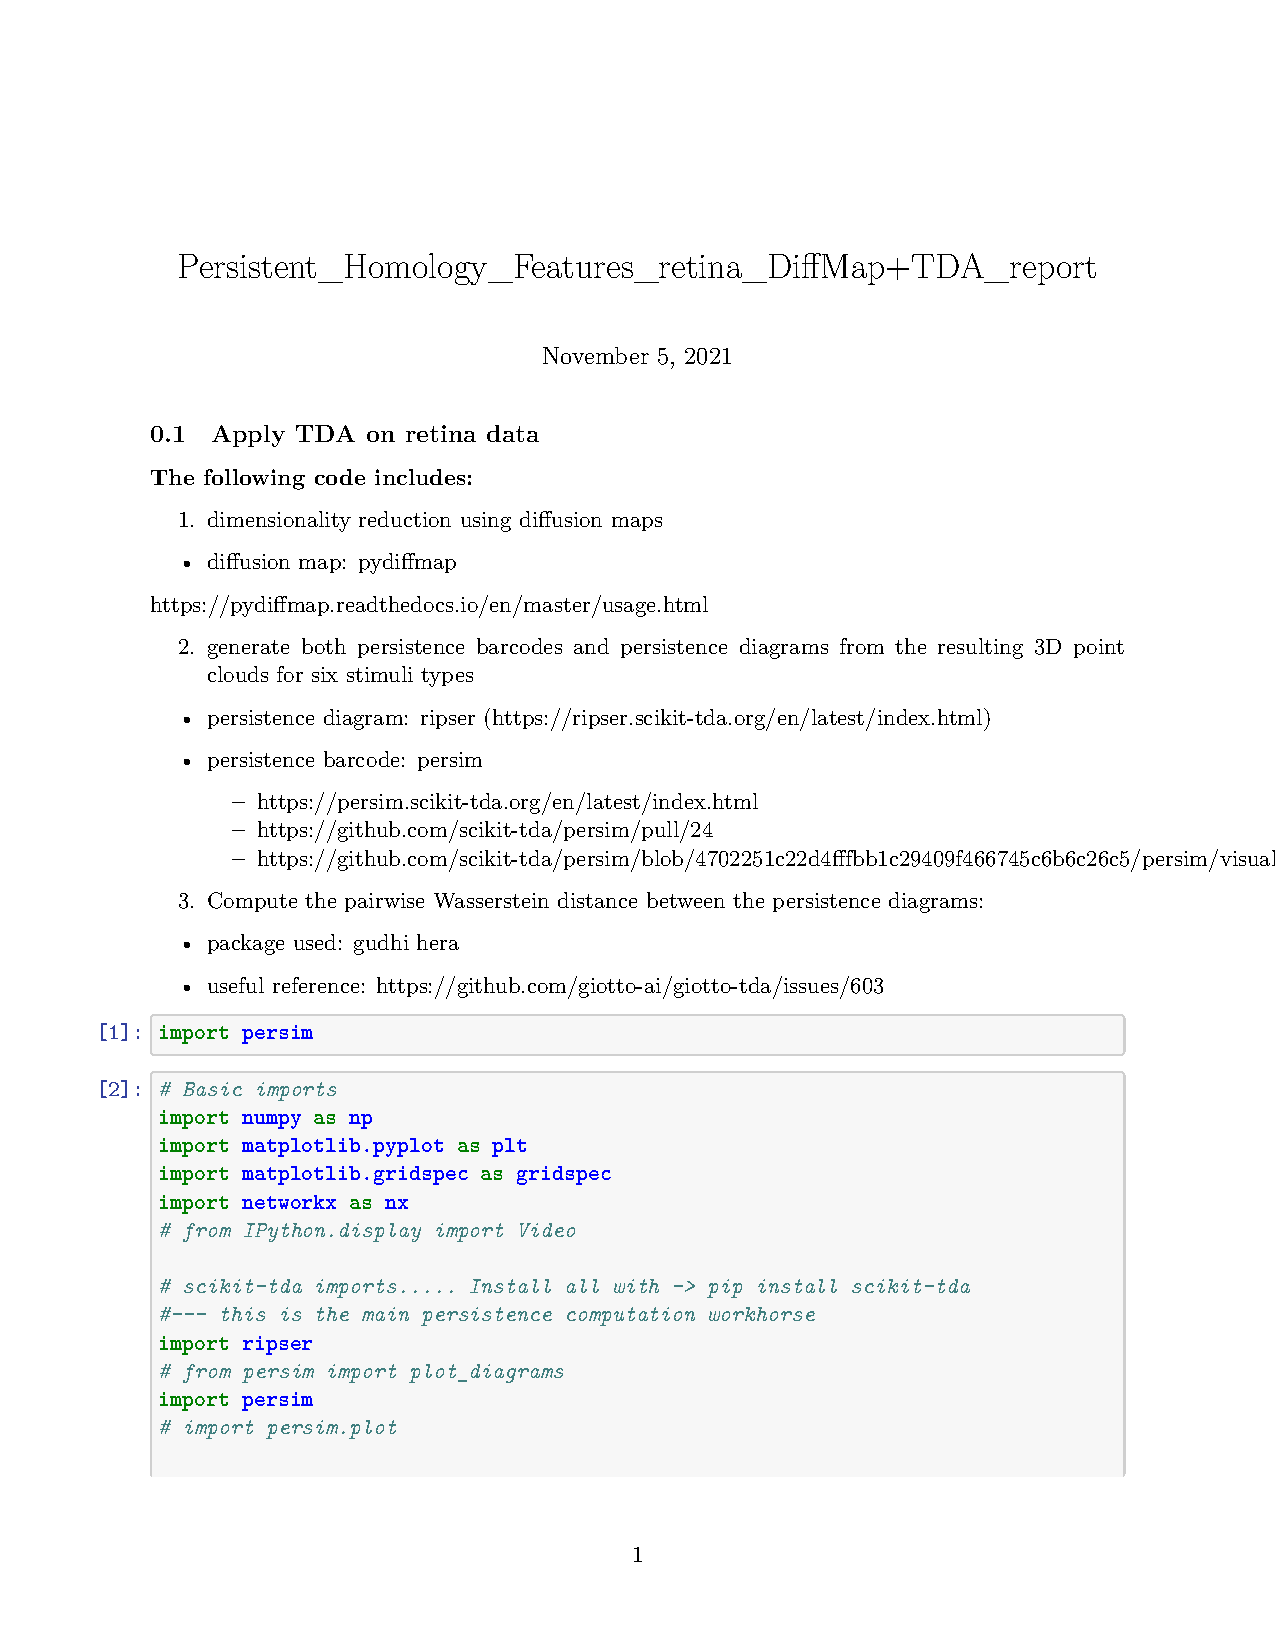
\includepdf[pages=-,pagecommand={},width=\textwidth]{Persistent_Homology_Features_retina_DiffMap+TDA_report.pdf}

\listoftables % Prints the list of tables
\label{lst:tabs}

\listoffigures % Prints the list of figures
\label{lst:figs}

%----------------------------------------------------------------------------------------
%	ABBREVIATIONS
%----------------------------------------------------------------------------------------

% \begin{abbreviations}{ll} % Include a list of abbreviations (a table of two columns)
%
% \textbf{LAH} & \textbf{L}ist \textbf{A}bbreviations \textbf{H}ere\\
% \textbf{WSF} & \textbf{W}hat (it) \textbf{S}tands \textbf{F}or\\
%
% \end{abbreviations}

%----------------------------------------------------------------------------------------

\end{document}
